\documentclass{standalone}
\usepackage{amsmath}
\usepackage{amssymb}
\usepackage{warpcol}
\usepackage{array}
\usepackage{esint}
\usepackage{subfig}
\usepackage{rotating}
\usepackage{booktabs}
\usepackage{paralist}
\usepackage{graphicx}
\usepackage{physics}
\usepackage{ucs}
\usepackage{indentfirst}
\usepackage{tikz}
\usepackage{colortbl}
\usepackage{xcolor}
\usepackage{xeCJK}
    \setCJKmainfont[BoldFont={Noto Serif CJK SC Bold},ItalicFont={FangSong}]{Noto Serif CJK SC}
    \setCJKsansfont[BoldFont={Noto Sans CJK SC Bold},ItalicFont={KaiTi}]{Noto Sans CJK SC}
    \setCJKmonofont[BoldFont={Noto Sans Mono CJK SC Bold}]{Noto Sans Mono CJK SC}

\DeclareUnicodeCharacter{"00B0}{\textdegree}
\DeclareUnicodeCharacter{"2103}{\textcelsius}

\pgfsetxvec{\pgfpoint{2.5em}{0}}
\pgfsetyvec{\pgfpoint{0}{2.5em}}

\usetikzlibrary{angles,patterns,datavisualization,plotmarks,arrows.meta,datavisualization.formats.functions,decorations.markings}

\begin{document}
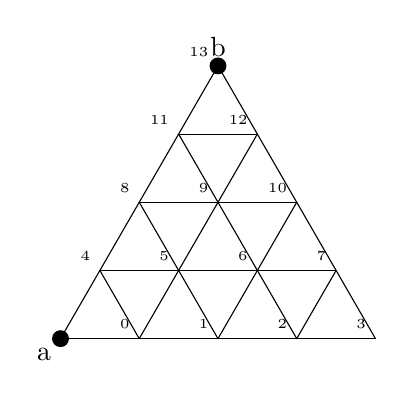
\begin{tikzpicture}
\foreach \i in {0,1,...,3}{
    \draw[line cap=round] (.5*\i-2, 3^.5*\i/2) -- (-.5*\i+2, 3^.5*\i/2);
    \draw[line cap=round] (-2.+\i, 0) -- (.5*\i, 3^.5*2-3^.5*\i/2);
    \draw[line cap=round] (2.-\i, 0) -- (-.5*\i, 3^.5*2-3^.5*\i/2);
}
\foreach \x/\y[count=\idx] in {
    -1/0, 0/0, 1/0, 2/0, -1.5/1, -.5/1, .5/1, 1.5/1,
    -1/2, 0/2, 1/2, -.5/3, .5/3, 0/4
}{
    \node[anchor=south east] at (\x, \y*3^.5/2) {\tiny\pgfmathparse{int(\idx-1)}\pgfmathresult};
}
\filldraw (-2, 0) node[below left] {a} circle (0.1);
\filldraw (0, 2*3^.5) node[above] {b} circle (0.1);
\end{tikzpicture}
\end{document}
